\centering
\hspace*{-0.01\textwidth}
\resizebox{0.5\textwidth}{!}{
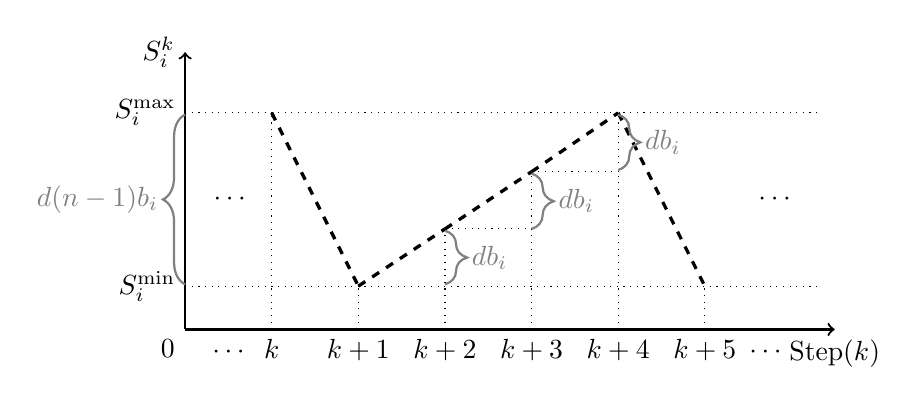
\begin{tikzpicture}[thick, scale=1.1][hbt!]
    % Axes
    \draw[->] (0,0) -- (7.5,0) node[below] {Step$(k)$};
    \draw[->] (0,0) -- (0,3.2) node[left] {$S_i^k$};

    % Horizontal dashed lines
    \draw[thin, dotted] (0,2.5) -- (7.3,2.5) node[anchor=east] at (0,2.5) {$S_i^{\max}$};
    \draw[thin, dotted] (0,0.5) -- (7.3,0.5) node[anchor=east] at (0,0.5) {$S_i^{\min}$};
    \draw[thin, dotted] (3,0.5+0.66) -- (4,0.5+0.66);
    \draw[thin, dotted] (4,0.5+0.66*2) -- (5,0.5+0.66*2);

    % Labels
    \node[below left] at (0,0) {$0$};
    \node[below] at (1,0) {$k$};
    \node[below] at (2,0) {$k+1$};
    \node[below] at (3,0) {$k+2$};
    \node[below] at (4,0) {$k+3$};
    \node[below] at (5,0) {$k+4$};
    \node[below] at (6,0) {$k+5$};
    \node[below] at (6.7,-0.07) {$\cdots$};
    \node[below] at (0.5,-0.07) {$\cdots$};

    % Dotted vertical lines for steps
    \draw[thin, dotted] (1,0) -- (1,2.5);
    \draw[thin, dotted] (2,0) -- (2,0.5);
    \draw[thin, dotted] (3,0) -- (3,0.5+0.66);
    \draw[thin, dotted] (4,0) -- (4,0.5+0.66*2);
    \draw[thin, dotted] (5,0) -- (5,2.5);
    \draw[thin, dotted] (6,0) -- (6,0.5);

    % Connecting dashed lines
    \draw[very thick, dashed] (1,2.5) -- (2,0.5);
    \draw[very thick, dashed] (2,0.5) -- (3,0.5+0.66);
    \draw[very thick, dashed] (3,0.5+0.66) -- (4,0.5+0.66*2);
    \draw[very thick, dashed] (4,0.5+0.66*2) -- (5,2.5);
    \draw[very thick, dashed] (5,2.5) -- (6,0.5);
    \node[right] at (6.5,1.5) {$\cdots$};
    \node[left] at (0.82,1.5) {$\cdots$};
    
    % Bracket
    \draw[decorate, decoration={brace, mirror, amplitude=8pt}, gray] 
        (0,2.48) -- (0,0.52) node[midway, left=6pt, gray] {$\textstyle d(n-1)b_i$};
    \draw[decorate, decoration={brace, mirror, amplitude=8pt}, gray]
        (3,0.52) -- (3,0.5+0.64) node[midway, right=6pt, gray] {$\textstyle db_i$};
    \draw[decorate, decoration={brace, mirror, amplitude=8pt}, gray]
        (4,0.5+0.66) -- (4,0.5+0.66*2-0.02) node[midway, right=6pt, gray] {$\textstyle db_i$};
    \draw[decorate, decoration={brace, mirror, amplitude=8pt}, gray]
        (5,0.5+0.66*2+0.02) -- (5,2.48) node[midway, right=6pt, gray] {$\textstyle db_i$};
\end{tikzpicture}
}
\caption{(Illustration of \Cref{theorem:lemma1}, $n=4$) This figure states that the row sum $S_i^k$ of the $i$-th row of the profit matrix $\profitList$ remains constant every $n$ steps. The fluctuations in the row sum are bounded by the difference $S_i^{\text{max}} - S_i^{\text{min}} = d(n-1)b_i$, where $S_i^{\text{max}}$ and $S_i^{\text{min}}$ denote the maximum and minimum row sums during the cycle. The diagram highlights the periodic nature of the row sum across steps and the incremental fluctuations $db_i$ within each step.}
\label{fig:fluctuations}